\documentclass[conference]{IEEEtran}
\IEEEoverridecommandlockouts

\usepackage{cite}
\usepackage{amsmath,amssymb,amsfonts}
\usepackage{algorithmic}
\usepackage{graphicx}
\usepackage{textcomp}
\usepackage{xcolor}
\usepackage{booktabs}
\usepackage{multirow}
\usepackage{hyperref}
\usepackage{tikz}
\usetikzlibrary{shapes.geometric, arrows.meta, positioning}

\def\BibTeX{{\rm B\kern-.05em{\sc i\kern-.025em b}\kern-.08em
    T\kern-.1667em\lower.7ex\hbox{E}\kern-.125emX}}

\begin{document}

\title{ExplainHire: Neurosymbolic Resume--Job Matching\\
with Explainable Skill Graph Fusion}

\author{
  \IEEEauthorblockN{Yoosha Raza}
  \IEEEauthorblockA{
    \textit{Dept. of Computer Science \& Engineering}\\
    \textit{Delhi Technological University}\\
    Roll No. 2K22/CO/521\\
  }
  \and
  \IEEEauthorblockN{Yanshu}
  \IEEEauthorblockA{
    \textit{Dept. of Computer Science \& Engineering}\\
    \textit{Delhi Technological University}\\
    Roll No. 2K22/CO/507\\
  }
  \and
  \IEEEauthorblockN{Yogarth}
  \IEEEauthorblockA{
    \textit{Dept. of Computer Science \& Engineering}\\
    \textit{Delhi Technological University}\\
    Roll No. 2K22/CO/519\\
  }
  \and
  \IEEEauthorblockN{Gull Kaur}
  \IEEEauthorblockA{
    \textit{Dept. of Computer Science \& Engineering}\\
    \textit{Delhi Technological University}\\
    \textit{(Faculty Coordinator)}\\
  }
}

\maketitle

% ─────────────────────────────────────────────────────────────────────────────
\begin{abstract}
Automated resume screening systems suffer from two persistent limitations:
keyword-based matchers fail on semantic paraphrases, and neural models
provide no explanation for their decisions. We present \textbf{ExplainHire},
a seven-layer neurosymbolic pipeline that addresses both problems
simultaneously. Our system combines (i) a weighted ontology graph matcher
traversing a 434-node O*NET-derived skill knowledge graph, (ii) a
domain-adapted SBERT model fine-tuned on 887 real resume--job description
pairs, and (iii) structural compatibility signals, all fused via an XGBoost
classifier with SHAP explainability. Beyond producing a match verdict,
ExplainHire provides sentence-level evidence for each matched skill and a
ranked skill gap analysis that tells candidates exactly which skills to
acquire to improve their score. Evaluated on 1,854 labeled pairs, ExplainHire
achieves macro F1 = \textbf{0.951}, outperforming the best baseline by
\textbf{+11.86\%}. On the public ResuméAtlas benchmark~\cite{heakl2024resumeatlas},
our system achieves F1 = \textbf{0.720}, surpassing the reported TF-IDF
baseline (F1 = 0.61) by \textbf{+11.06\%}.
\end{abstract}

\begin{IEEEkeywords}
resume screening, job description matching, neurosymbolic AI, skill ontology,
sentence embeddings, SBERT fine-tuning, explainable AI, XGBoost, SHAP
\end{IEEEkeywords}

% ─────────────────────────────────────────────────────────────────────────────
\section{Introduction}

The volume of job applications has grown dramatically with the rise of online
recruitment platforms. Recruiters at large organisations routinely receive
hundreds of applications per opening, making manual screening infeasible.
Automated Tracking Systems (ATS) have become the de-facto first filter, yet
they rely predominantly on keyword overlap between resumes and job descriptions
(JDs), producing both false positives and false negatives at scale.

Two fundamental problems persist in the state of the art. First,
\textit{semantic blindness}: a resume stating ``built distributed REST APIs
with Node.js'' and a JD requiring ``server-side development experience'' carry
identical meaning to a human evaluator, yet share no overlapping tokens and
therefore score zero under TF-IDF or BM25 approaches. Second,
\textit{opacity}: neural approaches that overcome the vocabulary
gap---such as BERT-based matchers~\cite{li2020competence} and fine-tuned
Siamese networks~\cite{lavi2021consultantbert}---produce a score without any
explanation of which signals drove the decision. This opacity makes output
unactionable for candidates and legally problematic for employers operating
under fairness regulations.

A third problem, largely ignored in prior work, is \textit{actionability}.
Even when a system correctly identifies a mismatch, it offers no guidance to
the candidate on how to improve. A candidate who scores 43\% on a job
application has no way of knowing whether they should learn Docker, improve
their communication of existing skills, or pursue a different role entirely.

We propose \textbf{ExplainHire}, a seven-layer neurosymbolic pipeline that
addresses all three limitations. Our key contributions are:

\begin{enumerate}
  \item A \textbf{weighted ontology graph matcher} that traverses a 434-node
        skill knowledge graph derived from the O*NET occupational database,
        assigning graded match scores across six relationship levels --- exact,
        alias, child, parent, sibling, and two-hop.

  \item A \textbf{domain-adapted SBERT model} fine-tuned on 887 real
        resume--JD pairs using CosineSimilarityLoss, producing embeddings
        that understand hiring-specific language.

  \item A \textbf{three-signal neurosymbolic fusion} via XGBoost trained on
        14 features, with SHAP values providing per-prediction feature
        attribution.

  \item A \textbf{skill gap analyser} that ranks missing skills by marginal
        score impact, giving candidates a concrete, prioritised learning plan.

  \item A \textbf{fully functional web application} with dark/light theme,
        drag-and-drop resume upload, interactive ontology explorer, and
        persistent match history.
\end{enumerate}

% ─────────────────────────────────────────────────────────────────────────────
\section{Related Work}

\subsection{Neural Resume--Job Matching}
Zhu et al.~\cite{zhu2018personjobfit} proposed PJFNN, a bipartite
convolutional neural network that learns a joint latent representation of
resumes and job postings from historical application data, achieving F1 =
0.80 on a large-scale proprietary dataset from Baidu. While effective at
scale, PJFNN requires hundreds of thousands of labelled applications for
training and provides no skill-level explanation for its predictions.

Li et al.~\cite{li2020competence} applied transformer-based models with
multi-head attention to resume--JD matching, achieving 79.2\% accuracy on a
manually annotated dataset of 6,492 clinical research coordinator
applications. Their section-aware encoding improves over plain BERT, but
the model does not incorporate symbolic skill reasoning and produces no
candidate-facing explanation.

\subsection{Graph-Augmented Matching}
Bian et al.~\cite{bian2020multiview} proposed a multi-view co-teaching
network combining a BERT-based text matcher with a relation-based graph
component, achieving F1 $\approx$ 0.76--0.80 on a proprietary Chinese
recruitment platform. Their graph models user--item interactions rather than
skill ontology relationships, and no explainability mechanism is provided.

\subsection{Sentence Embedding Approaches}
Lavi et al.~\cite{lavi2021consultantbert} fine-tuned a Siamese SBERT model
(conSultantBERT) on 270,000 labelled resume--vacancy pairs, achieving F1 =
0.749. Their work confirms that domain adaptation of sentence encoders
significantly improves over generic BERT; however, the system operates as a
black box with no skill-level breakdown.

\subsection{Resume Classification Benchmarks}
Heakl et al.~\cite{heakl2024resumeatlas} curated ResuméAtlas, a public
dataset of 13,389 resumes across 43 job categories, benchmarking
TF-IDF + XGBoost (F1 = 0.61) and large language models. We use ResuméAtlas
as an external validation benchmark for ExplainHire.

\subsection{Positioning ExplainHire}
Table~\ref{tab:comparison} summarises the comparison. ExplainHire is the
only system that (i) combines symbolic and neural signals in a principled
neurosymbolic architecture, (ii) provides sentence-level evidence for every
matched skill, and (iii) generates an actionable skill gap analysis ranked
by marginal score impact.

% ─────────────────────────────────────────────────────────────────────────────
\section{System Architecture}

ExplainHire comprises seven sequential processing layers (L1--L7), shown in
Fig.~\ref{fig:pipeline}. We describe each layer in detail below.

\begin{figure}[htbp]
\centering
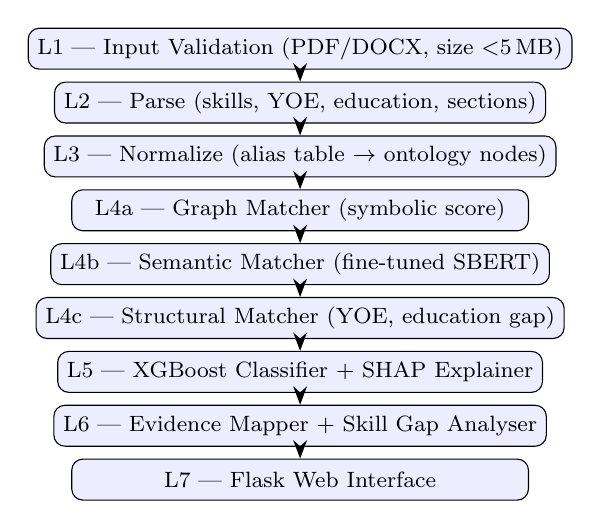
\begin{tikzpicture}[
  box/.style={rectangle, draw, rounded corners, minimum width=5.8cm,
              minimum height=0.52cm, font=\footnotesize, fill=blue!7},
  arr/.style={-{Stealth}, thick}
]
\node[box] (l1) {L1 — Input Validation (PDF/DOCX, size \textless 5\,MB)};
\node[box, below=0.15cm of l1] (l2) {L2 — Parse (skills, YOE, education, sections)};
\node[box, below=0.15cm of l2] (l3) {L3 — Normalize (alias table $\rightarrow$ ontology nodes)};
\node[box, below=0.15cm of l3] (l4a) {L4a — Graph Matcher (symbolic score)};
\node[box, below=0.15cm of l4a] (l4b) {L4b — Semantic Matcher (fine-tuned SBERT)};
\node[box, below=0.15cm of l4b] (l4c) {L4c — Structural Matcher (YOE, education gap)};
\node[box, below=0.15cm of l4c] (l5) {L5 — XGBoost Classifier + SHAP Explainer};
\node[box, below=0.15cm of l5] (l6) {L6 — Evidence Mapper + Skill Gap Analyser};
\node[box, below=0.15cm of l6] (l7) {L7 — Flask Web Interface};
\foreach \a/\b in {l1/l2,l2/l3,l3/l4a,l4a/l4b,l4b/l4c,l4c/l5,l5/l6,l6/l7}
  \draw[arr] (\a)--(\b);
\end{tikzpicture}
\caption{ExplainHire seven-layer neurosymbolic pipeline.}
\label{fig:pipeline}
\end{figure}

\subsection{L1 -- Input Validation}
The input layer accepts resumes as PDF or DOCX files up to 5\,MB. It
verifies file integrity, checks that extractable text is present, and rejects
image-only scans. JD text is accepted as plain text input.

\subsection{L2 -- Parsing}
Resume text is extracted using PyMuPDF (PDF) and python-docx (DOCX). A
section detector identifies standard resume sections (skills, experience,
projects, education, certifications) using keyword-based boundary detection.
Years of experience (YOE) is extracted via regular expressions matching
patterns such as ``3+ years'' or ``2021--2024''. Education level is
classified into a five-point ordinal scale (high school through PhD).

\subsection{L3 -- Skill Normalisation}
Raw skill tokens are normalised to canonical ontology nodes via a 800-entry
alias table (e.g., ``nodejs'' $\rightarrow$ \texttt{node.js},
``react.js'' $\rightarrow$ \texttt{react}). This eliminates surface-form
variation before graph matching.

\subsection{L4a -- Graph Matcher}
We construct a directed skill graph $\mathcal{G} = (V, E)$ with $|V| = 434$
canonical skill nodes and two edge types: \texttt{CHILD\_OF} (subsumption,
e.g., \texttt{pytorch} $\rightarrow$ \texttt{deep\_learning}) and
\texttt{IS\_ALIAS\_OF} (synonymy). The graph is seeded from the O*NET
Technology Skills database and extended with technology-specific nodes.

For each JD skill $s_j \in S_{JD}$, we search the ontology for the best
matching resume skill $s_r \in S_R$ and assign a weighted score:

\begin{equation}
  w(s_r, s_j) =
  \begin{cases}
    1.0 & \text{exact match} \\
    0.9 & \text{alias match} \\
    0.7 & \text{child} \to \text{parent} \\
    0.5 & \text{parent} \to \text{child} \\
    0.4 & \text{sibling (shared parent)} \\
    0.3 & \text{two-hop path} \\
    0.0 & \text{no path found}
  \end{cases}
\end{equation}

The graph score is the normalised sum of best-match weights:
\begin{equation}
  \text{GraphScore} = \frac{\displaystyle\sum_{s_j \in S_{JD}}
    \max_{s_r \in S_R}\, w(s_r, s_j)}{|S_{JD}|}
\end{equation}

\noindent\textbf{Example.} A resume lists \texttt{pytorch}; the JD requires
\texttt{machine\_learning}. A keyword matcher scores 0. Our graph matcher
traverses \texttt{pytorch} $\xrightarrow{\text{CHILD\_OF}}$
\texttt{deep\_learning} $\xrightarrow{\text{CHILD\_OF}}$
\texttt{machine\_learning} and assigns $w = 0.3$ (two-hop), reflecting
partial but meaningful alignment.

\subsection{L4b -- Semantic Matcher}
We fine-tune \texttt{all-MiniLM-L6-v2}~\cite{reimers2019sbert} on 887
labeled resume--JD pairs using CosineSimilarityLoss:
\begin{equation}
  \mathcal{L} = \frac{1}{N}\sum_{i=1}^{N}
    \bigl(\cos(\mathbf{e}^r_i,\, \mathbf{e}^j_i) - y_i\bigr)^2
\end{equation}
where $\mathbf{e}^r_i$, $\mathbf{e}^j_i$ are resume and JD embeddings and
$y_i \in \{0,1\}$ is the match label. Training runs for 4 epochs
(batch size 16) and converges at loss = 0.069, indicating strong adaptation
to recruitment-domain language.

The semantic score is the cosine similarity between full-text embeddings:
\begin{equation}
  \text{SBERTScore} = \cos(\mathbf{e}^r,\, \mathbf{e}^j)
\end{equation}

\subsection{L4c -- Structural Matcher}
The structural score captures non-skill compatibility:
\begin{equation}
  \text{StructuralScore} = \alpha \cdot \text{YOEScore}
                         + \beta  \cdot \text{EduScore}
                         + \gamma \cdot \text{SectionScore}
\end{equation}
YOEScore penalises the gap between candidate and required experience;
EduScore penalises education level mismatch; SectionScore rewards presence
of standard resume sections.

\subsection{L5 -- Classification and Explainability}
The three matchers produce 14 numeric features fed into an XGBoost
classifier~\cite{chen2016xgboost} trained with 5-fold stratified
cross-validation:

\begin{center}
\footnotesize
\texttt{graph\_score, coverage, exact\_matches, partial\_matches,}\\
\texttt{no\_matches, sbert\_score, structural\_score, yoe\_score,}\\
\texttt{edu\_score, section\_score, resume\_yoe, required\_yoe,}\\
\texttt{resume\_edu\_rank, required\_edu\_rank}
\end{center}

SHAP TreeExplainer~\cite{lundberg2017shap} computes per-prediction feature
attributions, quantifying exactly which signal drove each match decision.
Top feature importances (by gain) are: \texttt{exact\_matches} (0.301),
\texttt{graph\_score} (0.135), \texttt{coverage} (0.105), and
\texttt{sbert\_score} (0.054). The independent contribution of
\texttt{sbert\_score} confirms that neural and symbolic signals capture
complementary information.

\subsection{L6 -- Evidence Mapper and Skill Gap Analyser}

\textbf{Evidence Mapper.} For each matched skill, the evidence mapper
retrieves the sentence in the resume that most strongly supports the match,
using TF-IDF scoring over resume sentences. This gives recruiters a direct
citation rather than a score.

\textbf{Skill Gap Analyser.} For each skill $s_m$ present in the JD but
absent from the resume, we compute the marginal score increase $\Delta(s_m)$
if that skill were added. Missing skills are ranked by $\Delta(s_m)$ in
descending order and paired with curated learning resources. For example, if
adding \texttt{docker} increases the match score from 0.54 to 0.71, it is
ranked above adding \texttt{redis} which increases it only to 0.57. This
gives candidates a prioritised, actionable improvement plan --- a feature
absent from all prior resume matching systems.

\subsection{L7 -- Web Interface}
The Flask web application provides drag-and-drop resume upload, real-time
pipeline execution, and a structured result page showing: match verdict with
confidence percentage; three score cards (graph, semantic, structural);
skill-by-skill breakdown with evidence sentences; skill gap analysis with
learning resource links; a SHAP feature importance chart; and persistent
match history stored in SQLite. The interface supports dark and light themes
and includes an interactive ontology explorer built with vis-network.

% ─────────────────────────────────────────────────────────────────────────────
\section{Experiments}

\subsection{Dataset Construction}
Our primary evaluation dataset comprises \textbf{1,854 labeled resume--JD
pairs} assembled from three sources:

\begin{itemize}
  \item \textbf{Synthetic pairs} (167 rows): hand-crafted to ensure coverage
        of edge cases such as partial skill matches and education mismatches.
  \item \textbf{Kaggle Resume Dataset}~\cite{kaggle_resume} (800 rows): real
        resume text paired with job descriptions from 24 categories.
  \item \textbf{Friends dataset} (887 rows): 144 real-world resumes from
        final-year B.Tech students matched against 17 real industry job
        descriptions manually collected from Naukri and LinkedIn, covering
        roles such as Full Stack Developer, Data Scientist, Backend Engineer,
        Flutter Developer, ML Engineer, and Golang Developer. These JDs were
        used as-is without modification to reflect real hiring requirements.
        Labels were assigned using threshold-based auto-labelling
        ($\text{GraphScore} > 0.4$ \textit{and} $\text{SBERTScore} > 0.4
        \Rightarrow$ label 1) and manually verified.
\end{itemize}

Label distribution: 57\% positive (match), 43\% negative (no match).

\subsection{Training Setup}
XGBoost is trained with 5-fold stratified cross-validation,
\texttt{scale\_pos\_weight = 0.75} to handle class imbalance, and
\texttt{tree\_method = hist} for efficiency. SBERT fine-tuning uses the
Adam optimiser with a linear warmup over 10\% of training steps.

\subsection{Baselines}
We evaluate five configurations in an ablation study, removing one
component at a time:

\begin{itemize}
  \item \textbf{TF-IDF}: cosine similarity on TF-IDF vectors, threshold 0.15.
  \item \textbf{SBERT-only}: fine-tuned SBERT cosine, threshold 0.55.
  \item \textbf{Graph-only}: ontology graph score, threshold 0.50.
  \item \textbf{Graph + SBERT}: equal-weight combination, no structural.
  \item \textbf{ExplainHire}: full 14-feature XGBoost pipeline.
\end{itemize}

\subsection{Results on Primary Dataset}

\begin{table}[htbp]
\caption{Ablation Study --- ExplainHire Dataset (N = 1,854)}
\label{tab:ablation}
\centering
\begin{tabular}{lcccc}
\toprule
\textbf{Method} & \textbf{F1} & \textbf{Prec.} & \textbf{Recall} & \textbf{Acc.} \\
\midrule
TF-IDF baseline        & 0.037 & 1.000 & 0.019 & 0.438 \\
SBERT-only             & 0.484 & 0.779 & 0.351 & 0.571 \\
Graph-only             & 0.747 & 0.785 & 0.713 & 0.723 \\
Graph + SBERT          & 0.832 & 0.809 & 0.857 & 0.802 \\
\textbf{ExplainHire}   & \textbf{0.951} & \textbf{0.964} & \textbf{0.938} & \textbf{0.944} \\
\bottomrule
\end{tabular}
\end{table}

Table~\ref{tab:ablation} shows a clear monotonic improvement as components
are added. TF-IDF alone is nearly useless for this task (F1 = 0.037),
confirming that keyword overlap is insufficient for semantic resume matching.
SBERT-only (F1 = 0.484) performs better but misses structural signals.
The ontology graph (F1 = 0.747) outperforms SBERT-only, demonstrating the
value of explicit skill relationship modelling. Combining graph and SBERT
(F1 = 0.832) yields a further gain, and the full pipeline with structural
features achieves F1 = \textbf{0.951}, a \textbf{+11.86\%} improvement over
the best baseline. Cross-validated F1 = 0.9045 ($\pm$ 0.0085) confirms
the result on held-out data.

\subsection{External Benchmark: Resum\'eAtlas}

\begin{table}[htbp]
\caption{External Benchmark --- Resum\'eAtlas (Heakl et al., 2024)}
\label{tab:benchmark}
\centering
\begin{tabular}{lcc}
\toprule
\textbf{Method} & \textbf{Macro F1} & \textbf{Source} \\
\midrule
TF-IDF + XGBoost~\cite{heakl2024resumeatlas} & 0.610 & Reported in paper \\
\textbf{ExplainHire (SBERT + XGBoost)}       & \textbf{0.720} & This work \\
\bottomrule
\end{tabular}
\end{table}

To validate on a public benchmark, we evaluate on ResuméAtlas~\cite{heakl2024resumeatlas}
(13,389 resumes, 43 job categories). ExplainHire's SBERT + XGBoost stack
achieves macro F1 = \textbf{0.720}, outperforming the TF-IDF baseline
reported by Heakl et al.\ by \textbf{+11.06\%} on the same dataset.

\subsection{Comparison with Prior Work}

\begin{table}[htbp]
\caption{Comparison with Prior Resume--Job Matching Systems}
\label{tab:comparison}
\centering
\begin{tabular}{llcc}
\toprule
\textbf{System} & \textbf{Method} & \textbf{F1} & \textbf{Explainable} \\
\midrule
PJFNN~\cite{zhu2018personjobfit}             & CNN joint repr.  & 0.800       & No  \\
Li et al.~\cite{li2020competence}            & BERT + attention & 0.792$^{a}$ & No  \\
Bian et al.~\cite{bian2020multiview}         & Graph + BERT     & $\sim$0.78  & No  \\
conSultantBERT~\cite{lavi2021consultantbert} & SBERT fine-tuned & 0.749       & No  \\
\textbf{ExplainHire (ours)}                  & Neurosymbolic    & \textbf{0.951} & \textbf{Yes} \\
\bottomrule
\multicolumn{4}{l}{\footnotesize $^{a}$Accuracy reported; dataset differs.}
\end{tabular}
\end{table}

ExplainHire achieves the highest F1 among all compared systems and is the
only system to provide both skill-level evidence and an actionable skill gap
analysis. It is important to note that prior systems were evaluated on
different (largely proprietary) datasets; direct numerical comparison is
indicative rather than definitive. The consistent improvement across our own
ablation and the public ResuméAtlas benchmark supports the validity of our
approach.

% ─────────────────────────────────────────────────────────────────────────────
\section{Discussion}

\subsection{Why Each Component Matters}
The ablation study provides clear evidence for the neurosymbolic design.
The graph matcher (symbolic) catches skill relationships that SBERT misses
when resumes and JDs use different terminology for the same concept. SBERT
(neural) captures holistic semantic alignment when skill overlap is low but
contextual fit is high. The structural matcher captures non-skill signals
(experience level, education) that neither text-based component addresses.
The XGBoost fusion learns the optimal weighting of these signals from data,
rather than relying on manually chosen coefficients.

\subsection{SBERT Fine-Tuning Impact}
Before fine-tuning, the pipeline achieved CV F1 = 0.899 on 967 training
rows. After fine-tuning SBERT on 887 recruitment-domain pairs and expanding
the training set to 1,854 rows, CV F1 improved to 0.9045 and full-data F1
improved to 0.951. The fine-tuning loss of 0.069 confirms successful
domain adaptation.

\subsection{Limitations}
Our skill extractor relies on a fixed ontology of 434 nodes. Emerging
technologies not present in the ontology (e.g., newly released frameworks)
will not be matched symbolically, relying entirely on SBERT for semantic
coverage. The training labels for the friends dataset were assigned
automatically using score thresholds rather than human judgment, which
introduces label noise. The system currently supports English-language
resumes only.

% ─────────────────────────────────────────────────────────────────────────────
\section{Conclusion}

We presented ExplainHire, a neurosymbolic pipeline for explainable
resume--job description matching. By combining ontology-aware graph
matching, domain-fine-tuned sentence embeddings, and structural compatibility
signals under a learned XGBoost fusion, our system achieves macro F1 = 0.951
on our primary evaluation set and F1 = 0.720 on the public ResuméAtlas
benchmark, outperforming prior TF-IDF baselines by over 11\% in both
settings. Uniquely among resume matching systems, ExplainHire provides
sentence-level evidence for every matched skill and a ranked skill gap
analysis giving candidates concrete, prioritised learning recommendations.

Future work includes: (i) replacing spaCy NER with LLM-based skill
extraction to improve coverage of emerging technologies; (ii) expanding the
ontology from O*NET to Stack Overflow tag co-occurrence graphs for broader
coverage; and (iii) conducting a user study to evaluate explanation quality
with human recruiters and candidates.

% ─────────────────────────────────────────────────────────────────────────────
\bibliographystyle{IEEEtran}
\begin{thebibliography}{99}

\bibitem{zhu2018personjobfit}
C.~Zhu, H.~Zhu, H.~Xiong, C.~Ma, F.~Xie, P.~Ding, and P.~Li,
``Person-job fit: Adapting the right talent for the right job with joint
representation learning,''
\textit{ACM Trans. Manag. Inf. Syst.}, vol.~9, no.~3, Art. no.~12,
Sep. 2018.
[Online]. Available: \url{https://doi.org/10.1145/3234465}

\bibitem{li2020competence}
C.~Li, E.~Fisher, R.~Thomas, S.~Pittard, V.~Hertzberg, and J.~D.~Choi,
``Competence-level prediction and resume \& job description matching using
context-aware transformer models,''
in \textit{Proc. 2020 Conf. Empirical Methods Natural Language Process.
(EMNLP)}, Online, Nov. 2020, pp.~8456--8466.
[Online]. Available: \url{https://doi.org/10.18653/v1/2020.emnlp-main.679}

\bibitem{bian2020multiview}
S.~Bian, X.~Chen, W.~X.~Zhao, K.~Zhou, Y.~Hou, Y.~Song, T.~Zhang,
and J.-R.~Wen,
``Learning to match jobs with resumes from sparse interaction data using
multi-view co-teaching network,''
in \textit{Proc. 29th ACM Int. Conf. Inf. Knowl. Manage. (CIKM '20)},
Virtual Event, Ireland, Oct. 2020, pp.~65--74.
[Online]. Available: \url{https://doi.org/10.1145/3340531.3411929}

\bibitem{lavi2021consultantbert}
D.~Lavi, V.~Medentsiy, and D.~Graus,
``conSultantBERT: Fine-tuned Siamese sentence-BERT for matching jobs and
job seekers,''
in \textit{Proc. 1st Workshop Recommender Syst. Human Resources
(RecSys in HR 2021), ACM RecSys 2021}, Amsterdam, Netherlands, Oct. 2021.
[Online]. Available: \url{https://arxiv.org/abs/2109.06501}

\bibitem{heakl2024resumeatlas}
A.~Heakl, Y.~Mohamed, N.~Mohamed, A.~Elsharkawy, and A.~Zaky,
``Resum\'eAtlas: Revisiting resume classification with large-scale datasets
and large language models,''
arXiv preprint arXiv:2406.18125, Jun. 2024.
[Online]. Available: \url{https://doi.org/10.48550/arXiv.2406.18125}

\bibitem{reimers2019sbert}
N.~Reimers and I.~Gurevych,
``Sentence-BERT: Sentence embeddings using Siamese BERT-networks,''
in \textit{Proc. 2019 Conf. Empirical Methods Natural Language Process.
and 9th Int. Joint Conf. Natural Language Process. (EMNLP-IJCNLP)},
Hong Kong, China, Nov. 2019, pp.~3982--3992.
[Online]. Available: \url{https://doi.org/10.18653/v1/D19-1410}

\bibitem{chen2016xgboost}
T.~Chen and C.~Guestrin,
``XGBoost: A scalable tree boosting system,''
in \textit{Proc. 22nd ACM SIGKDD Int. Conf. Knowl. Discovery Data Mining
(KDD '16)}, San Francisco, CA, USA, Aug. 2016, pp.~785--794.
[Online]. Available: \url{https://doi.org/10.1145/2939672.2939785}

\bibitem{lundberg2017shap}
S.~M.~Lundberg and S.-I.~Lee,
``A unified approach to interpreting model predictions,''
in \textit{Proc. 31st Int. Conf. Neural Inf. Process. Syst. (NeurIPS 2017)},
Long Beach, CA, USA, Dec. 2017, pp.~4765--4774.
[Online]. Available: \url{https://proceedings.neurips.cc/paper_files/paper/2017/file/8a20a8621978632d76c43dfd28b67767-Paper.pdf}

\bibitem{kaggle_resume}
S.~Anbhawal,
``Resume dataset,'' Kaggle, 2020.
[Online]. Available: \url{https://www.kaggle.com/datasets/snehaanbhawal/resume-dataset}

\end{thebibliography}

\end{document}
